\subsection{Mine}\label{sec:lehrpfad_conversions}
\begin{figure}[H]
    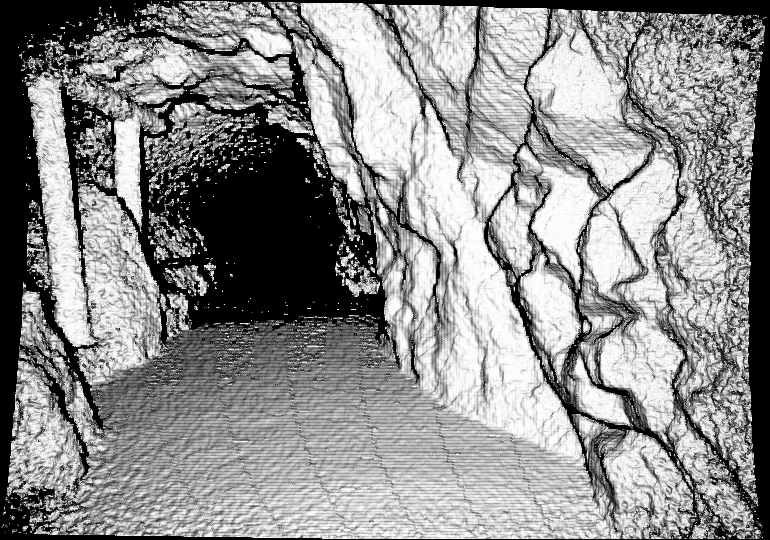
\includegraphics[width=0.25\linewidth]{chapter06/results/conv_images/lehrpfad/flexion/raw/0000.png}%
    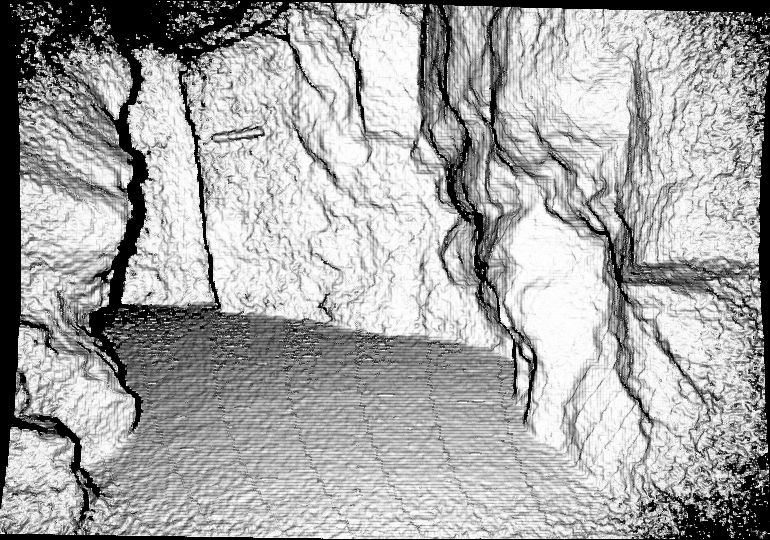
\includegraphics[width=0.25\linewidth]{chapter06/results/conv_images/lehrpfad/flexion/raw/0090.png}%
    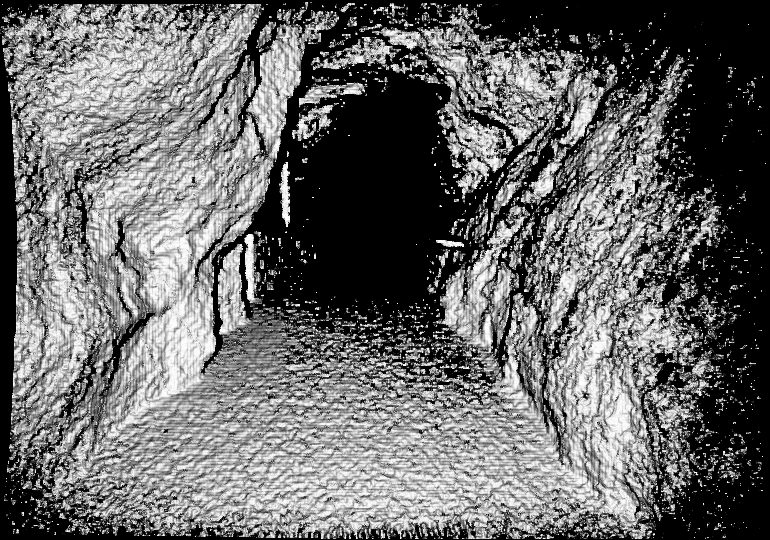
\includegraphics[width=0.25\linewidth]{chapter06/results/conv_images/lehrpfad/flexion/raw/0180.png}%
    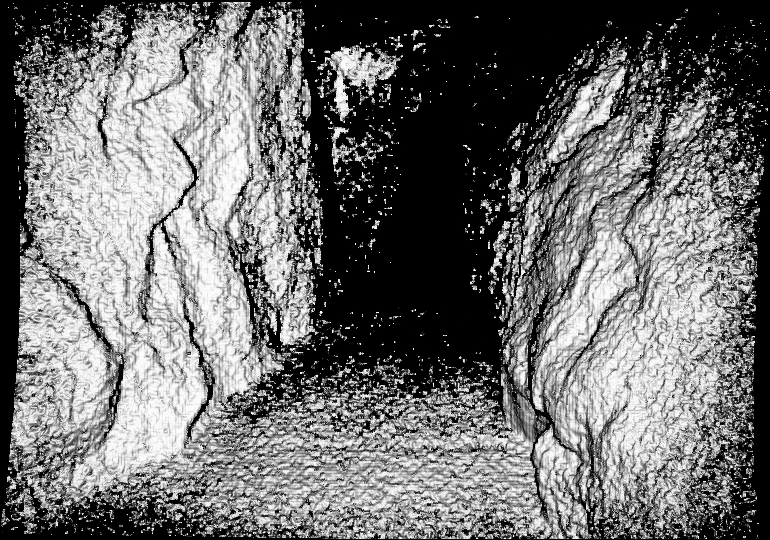
\includegraphics[width=0.25\linewidth]{chapter06/results/conv_images/lehrpfad/flexion/raw/0270.png}\\
    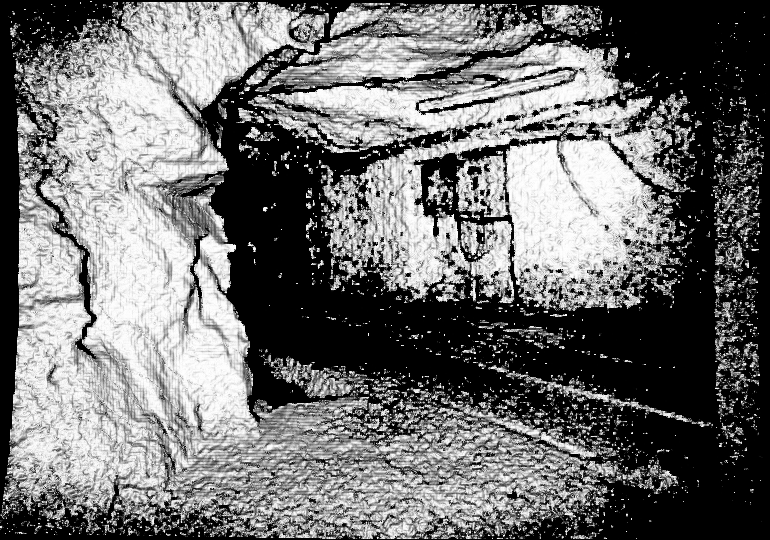
\includegraphics[width=0.25\linewidth]{chapter06/results/conv_images/lehrpfad/flexion/raw/0360.png}%
    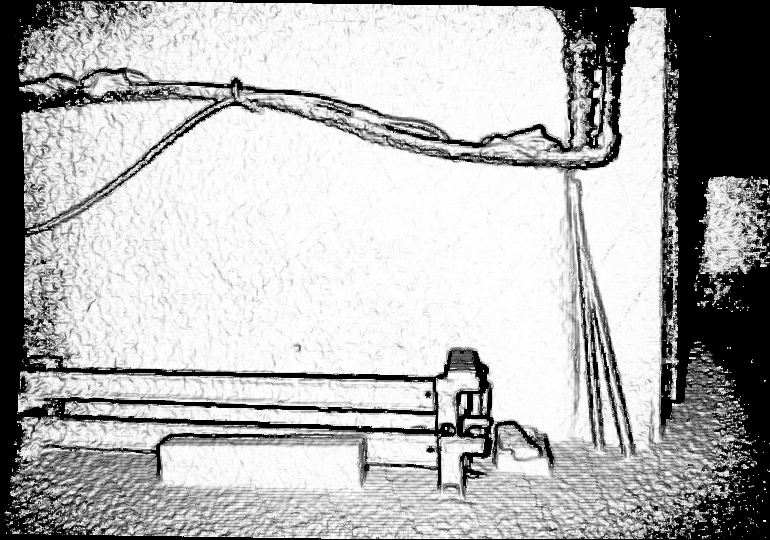
\includegraphics[width=0.25\linewidth]{chapter06/results/conv_images/lehrpfad/flexion/raw/0450.png}%
    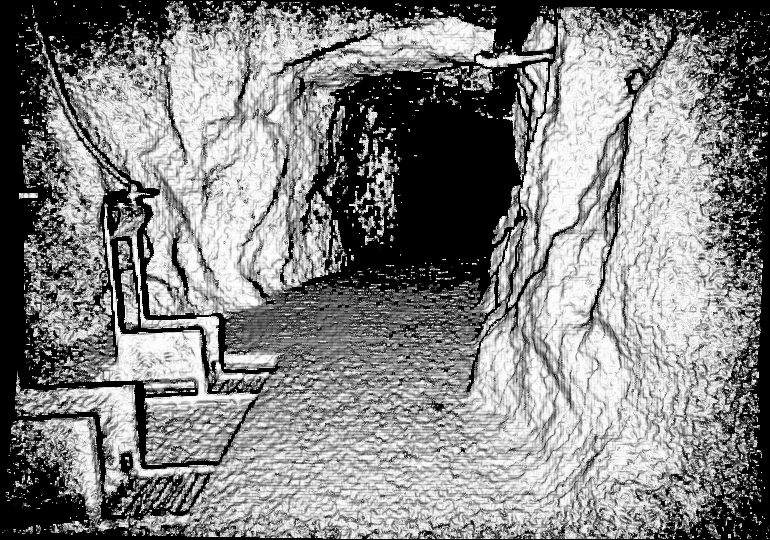
\includegraphics[width=0.25\linewidth]{chapter06/results/conv_images/lehrpfad/flexion/raw/0540.png}%
    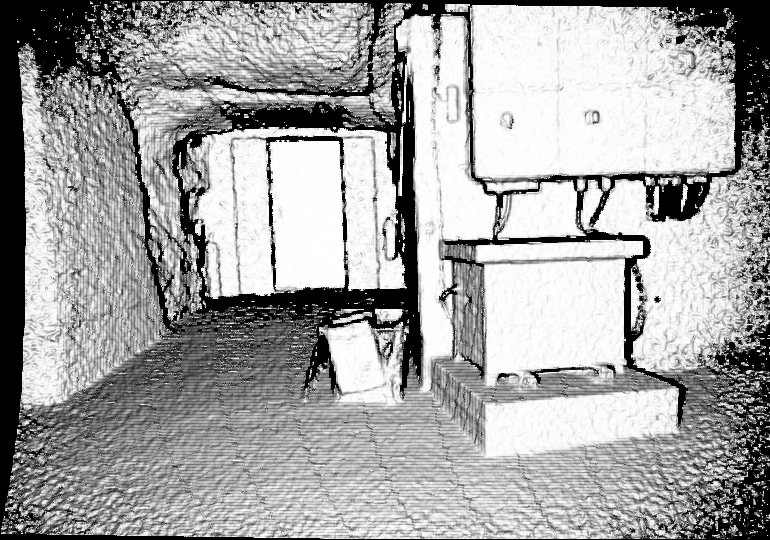
\includegraphics[width=0.25\linewidth]{chapter06/results/conv_images/lehrpfad/flexion/raw/0630.png}\\
    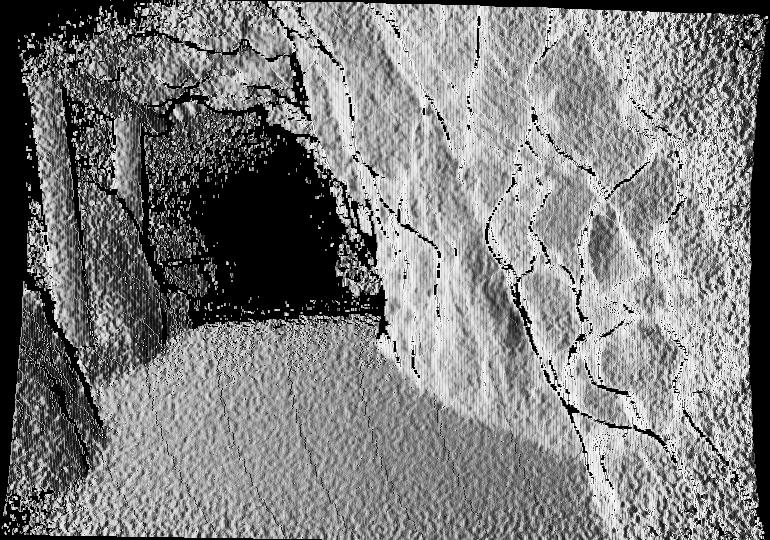
\includegraphics[width=0.25\linewidth]{chapter06/results/conv_images/lehrpfad/bearing/raw/0000.png}%
    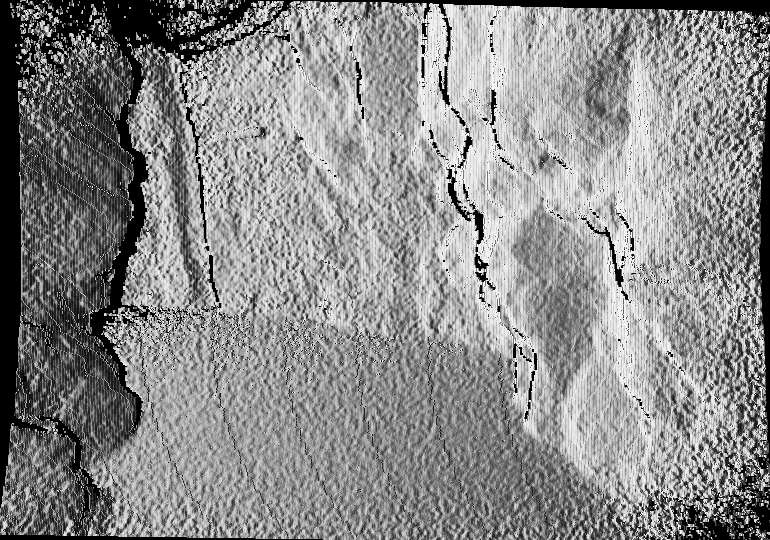
\includegraphics[width=0.25\linewidth]{chapter06/results/conv_images/lehrpfad/bearing/raw/0090.png}%
    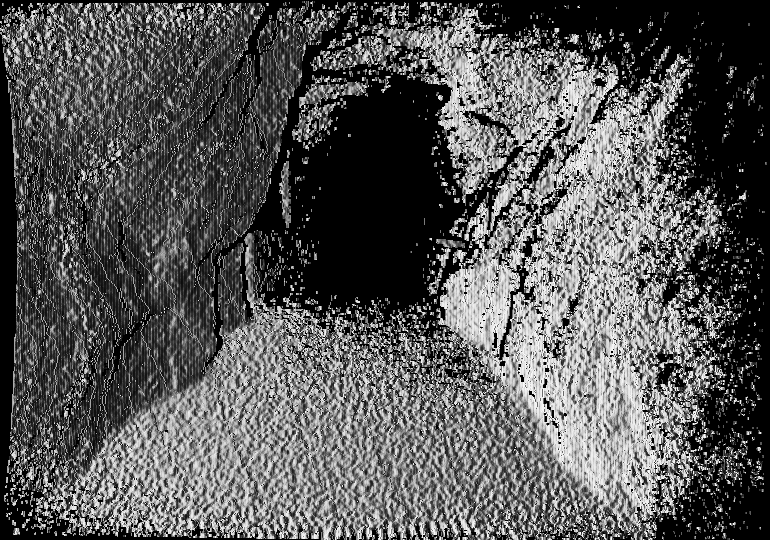
\includegraphics[width=0.25\linewidth]{chapter06/results/conv_images/lehrpfad/bearing/raw/0180.png}%
    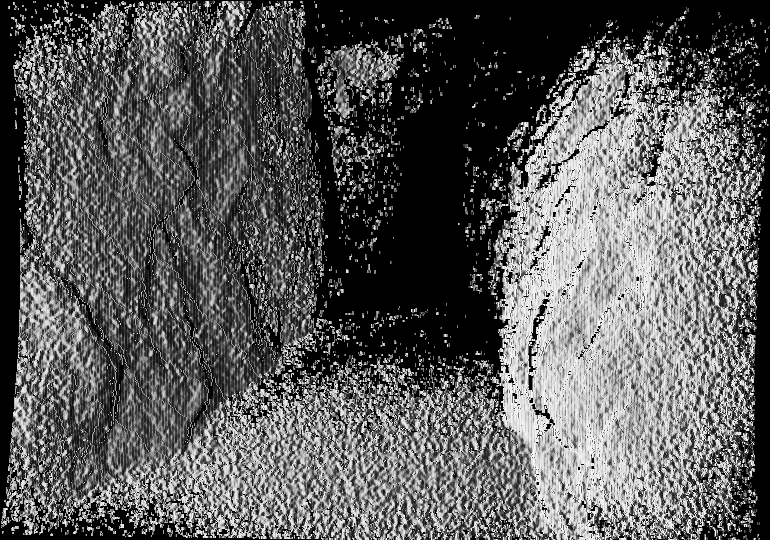
\includegraphics[width=0.25\linewidth]{chapter06/results/conv_images/lehrpfad/bearing/raw/0270.png}\\
    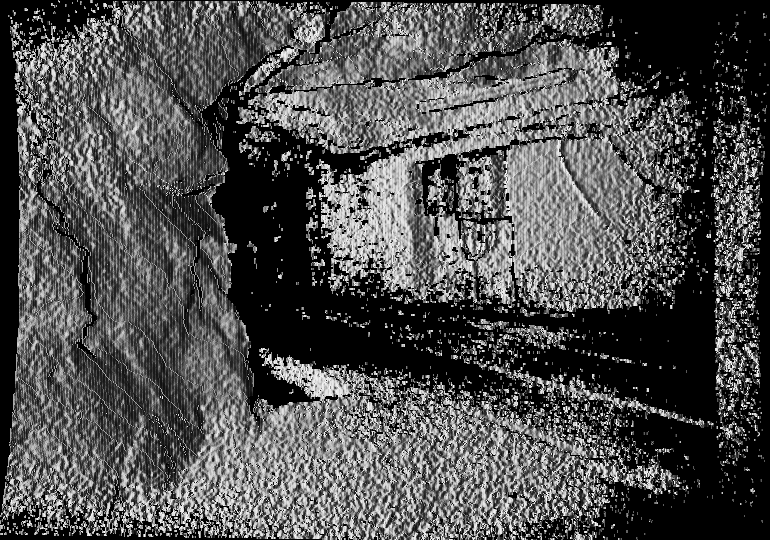
\includegraphics[width=0.25\linewidth]{chapter06/results/conv_images/lehrpfad/bearing/raw/0360.png}%
    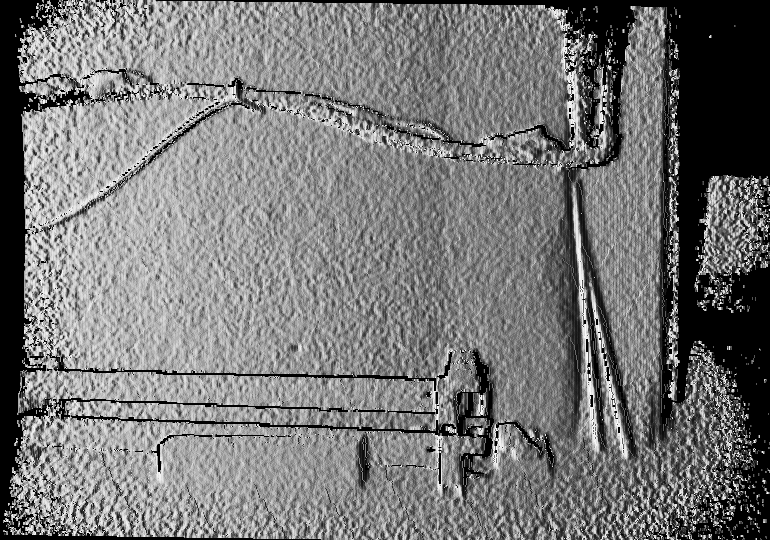
\includegraphics[width=0.25\linewidth]{chapter06/results/conv_images/lehrpfad/bearing/raw/0450.png}%
    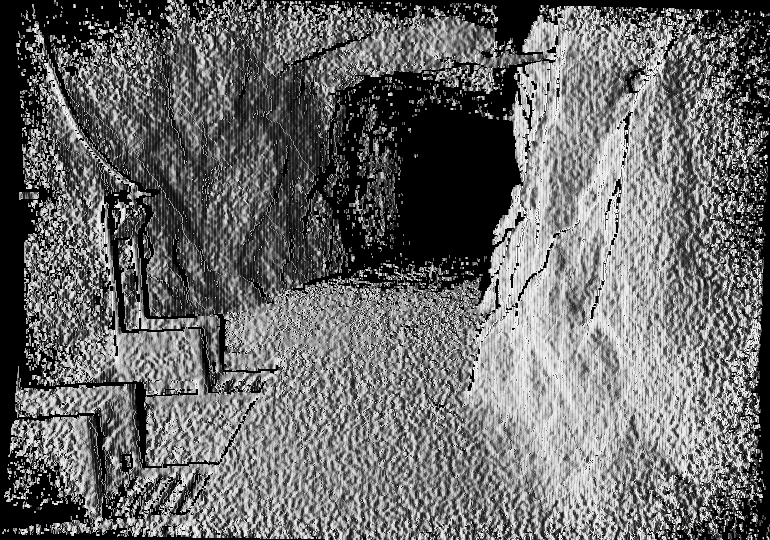
\includegraphics[width=0.25\linewidth]{chapter06/results/conv_images/lehrpfad/bearing/raw/0540.png}%
    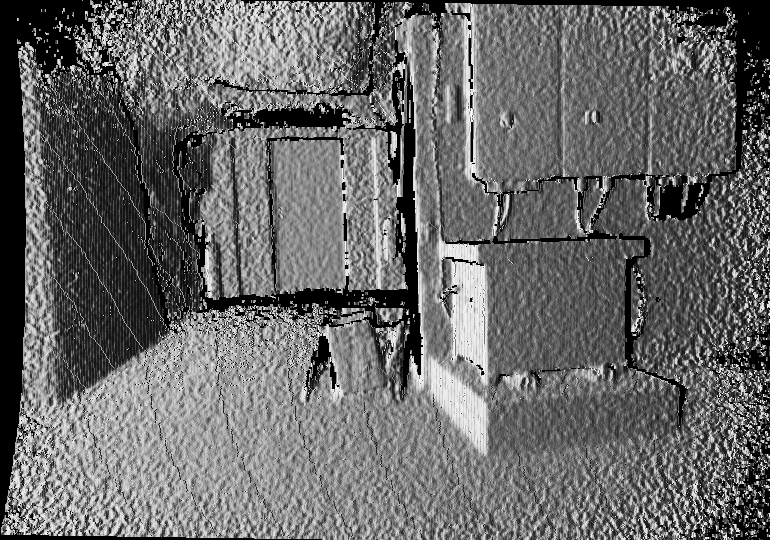
\includegraphics[width=0.25\linewidth]{chapter06/results/conv_images/lehrpfad/bearing/raw/0630.png}%
    \caption[Examples of the \emph{Mine} feature image conversions]{Example \glspl{flexion-image} and \glspl{bearing-angle-image} of the \emph{Mine} dataset without any filtering.}
\end{figure}
\begin{figure}[H]
    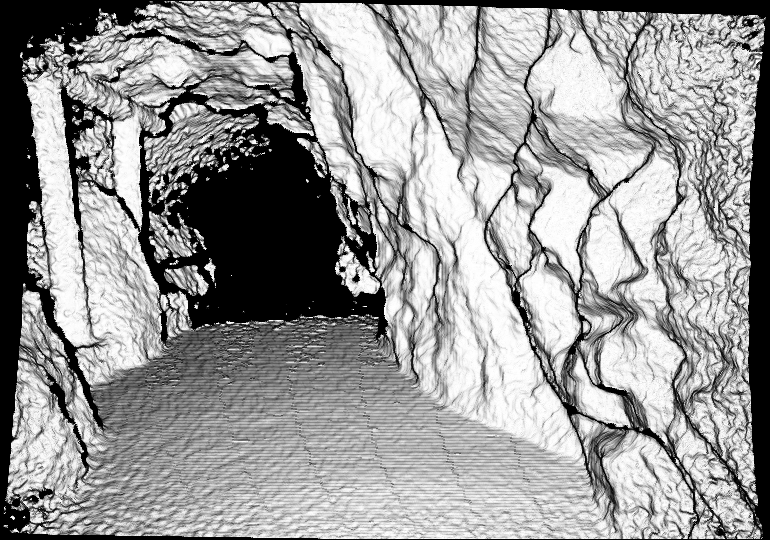
\includegraphics[width=0.25\linewidth]{chapter06/results/conv_images/lehrpfad/flexion/mb/0000.png}%
    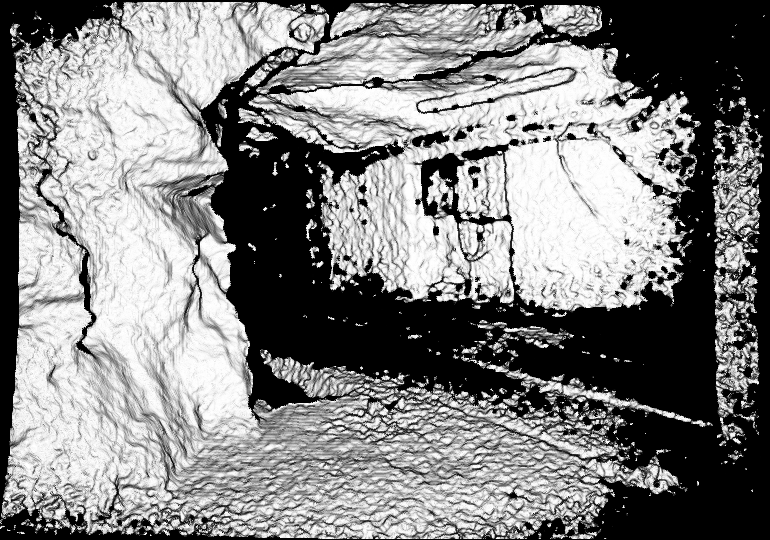
\includegraphics[width=0.25\linewidth]{chapter06/results/conv_images/lehrpfad/flexion/mb/0360.png}%
    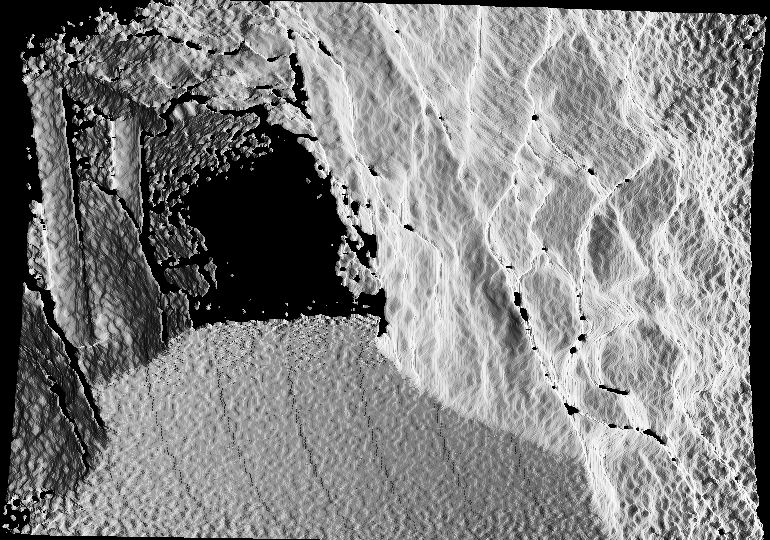
\includegraphics[width=0.25\linewidth]{chapter06/results/conv_images/lehrpfad/bearing/mb/0000.png}%
    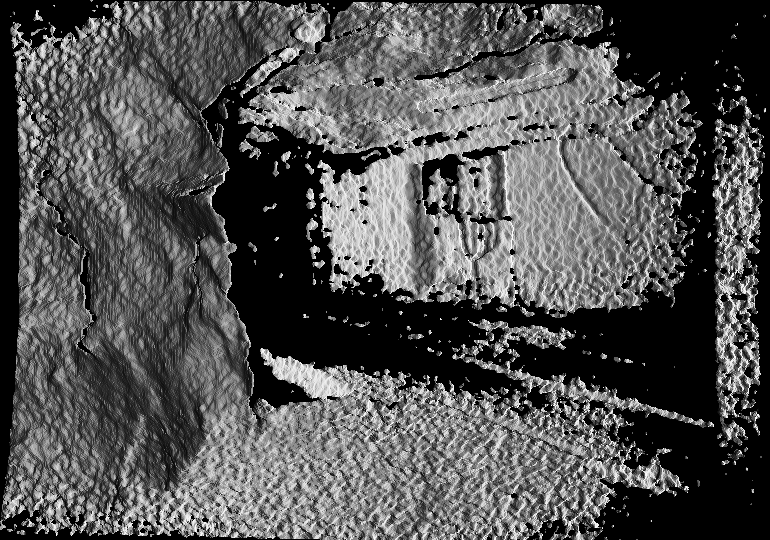
\includegraphics[width=0.25\linewidth]{chapter06/results/conv_images/lehrpfad/bearing/mb/0360.png}%
    \caption{Effect of median blur filtering on the \emph{Mine} data.}
\end{figure}
\begin{figure}[H]
    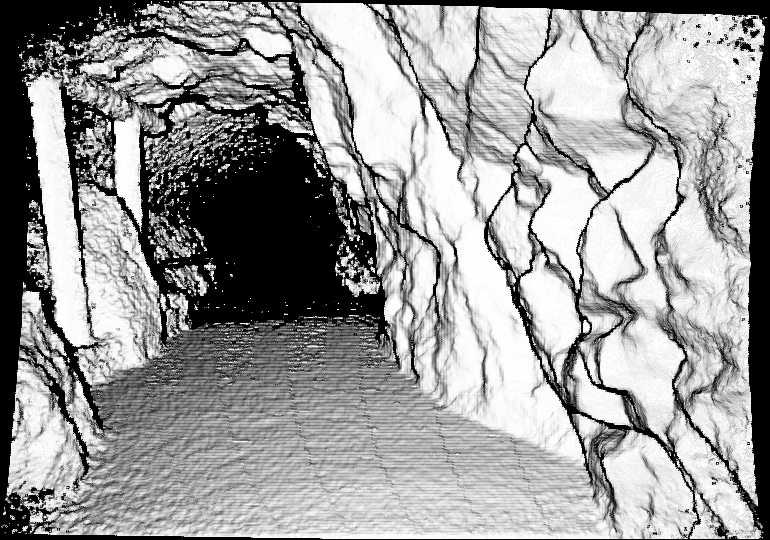
\includegraphics[width=0.25\linewidth]{chapter06/results/conv_images/lehrpfad/flexion/bl/0000.png}%
    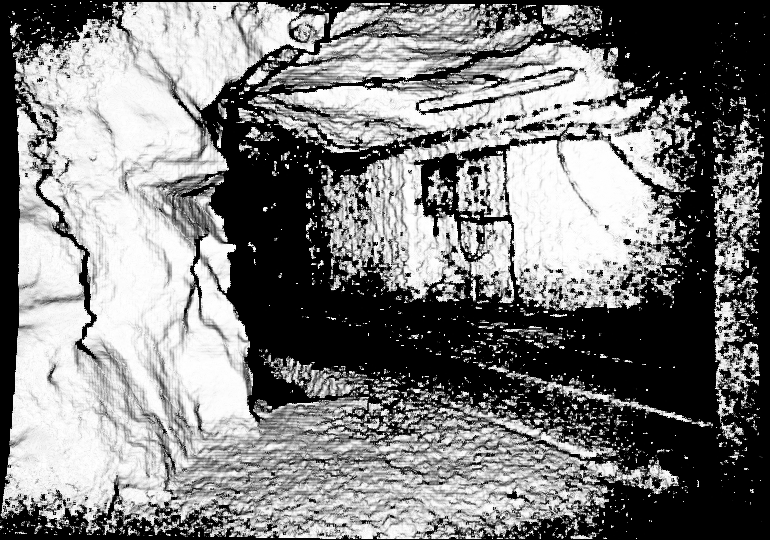
\includegraphics[width=0.25\linewidth]{chapter06/results/conv_images/lehrpfad/flexion/bl/0360.png}%
    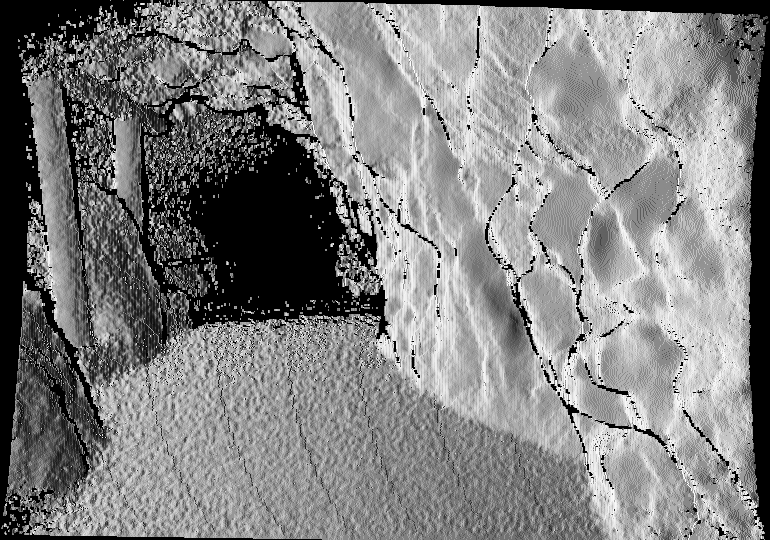
\includegraphics[width=0.25\linewidth]{chapter06/results/conv_images/lehrpfad/bearing/bl/0000.png}%
    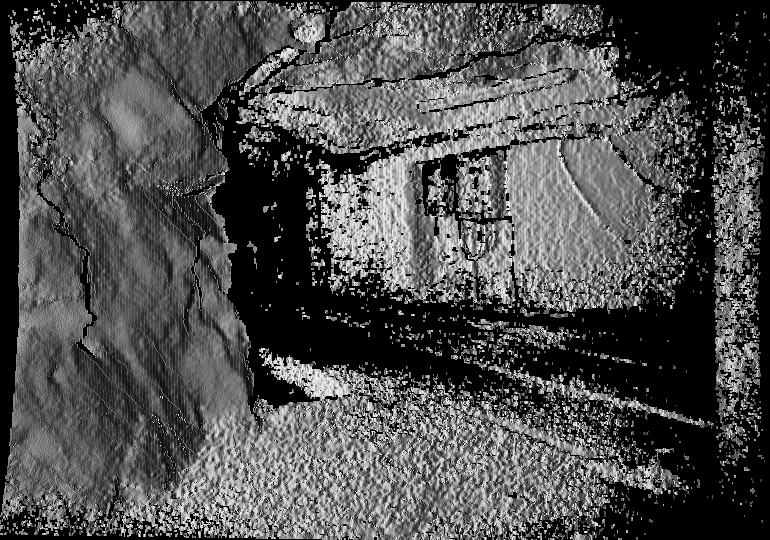
\includegraphics[width=0.25\linewidth]{chapter06/results/conv_images/lehrpfad/bearing/bl/0360.png}%
    \caption{Effect of bilateral filtering on the \emph{Mine} data.}
\end{figure}
